\documentclass[11pt,a4paper]{article}
\usepackage[utf8]{inputenc}
\usepackage{amsmath,amssymb}
\usepackage{graphicx}
\usepackage{booktabs}
\usepackage{geometry}
\usepackage{float}
\geometry{margin=1in}
\setlength{\emergencystretch}{3em}

\title{\textbf{Kimchi Premium and Triangular Arbitrage Dislocation Dynamics}\\Draft v2}
\author{Songgun Lee \\ \textit{Department of Physics, University of California, Santa Barbara}}
\date{April 2026 (Preprint)}

\begin{document}
\maketitle

\begin{abstract}
This paper studies whether external macro dislocation (kimchi premium) induces exploitable internal inefficiency in a fiat-isolated crypto exchange. Using 141,200 minute-level observations (ADA, DOGE, ETH, SOL, XRP), forward and reverse triangular routes are analyzed separately and then aggregated through optimistic best-direction operators. Under an Upbit-consistent mixed taker fee barrier of $V_0=0.35\%$, no global best-minute event exceeds the execution threshold in the observed sample. Even at the looser $0.15\%$ threshold, exceedance frequency remains near-zero. The evidence indicates high short-horizon internal market efficiency under practical fee-aware execution constraints, with dislocations behaving as transient phase-like states rather than persistent retail-exploitable arbitrage windows.
\end{abstract}

\tableofcontents
\newpage

\section{Introduction}
\subsection{Motivation}
Most discussions of crypto arbitrage begin from a frictionless premise: if a cross-venue price gap exists, capital should flow until the gap closes. In practice, this logic is incomplete for retail and semi-systematic execution, because tradability depends on market-specific frictions that are not small perturbations but first-order constraints. In KRW-linked markets, the kimchi premium is visible as a macro dislocation signal, yet converting that signal into realized triangular profit requires surviving fee layers, spread crossing, timing mismatch, and route consistency at minute granularity.

This paper studies the dislocation question in the specific context where these frictions are structurally binding: a fiat-isolated exchange environment with asymmetric route costs. Rather than asking whether dislocation exists in principle, we ask whether it survives a realistic execution barrier often enough to be considered an exploitable state. The distinction is central. A market can display persistent premium dispersion while still behaving as highly efficient for executable internal arbitrage once route-level costs are imposed.

The empirical strategy therefore treats kimchi premium and triangular net-profit as coupled but non-equivalent state variables. Kimchi premium captures macro divergence pressure between KRW and global crypto pricing, while triangular net-profit captures local convertibility efficiency inside the exchange graph. If market structure is truly efficient at the minute horizon, high macro dislocation should not systematically translate into fee-cleared internal edge. Testing this mapping, rather than merely describing premium levels, is the core motivation of the study.

\subsection{Research Question}
The central research question is:

\emph{Does external macro dislocation (kimchi-premium volatility) induce exploitable internal microstructural inefficiency within a fiat-isolated order book?}

To make this test operational, ``exploitable'' is defined in fee-aware terms rather than sign-only profitability. Specifically, the relevant object is the frequency of events where route-level net profit exceeds a pre-specified execution barrier $V_0$, with additional sensitivity checks at stricter thresholds. This framing prevents false positives that arise when positive but non-executable micro-gains are treated as arbitrage opportunities.

\subsection{Contribution}
Relative to dashboard-style premium tracking, this paper makes four concrete contributions. First, it formalizes a route-level, fee-consistent execution barrier grounded in the Upbit schedule and uses that barrier as the primary test statistic for tradable edge. Second, it introduces a hierarchical analysis protocol that separates directional routes and then aggregates in two stages (best-per-asset-per-minute, then global best-per-minute), allowing optimistic upper-envelope testing without conflating route asymmetry. Third, it reports explicit tail-event frequencies above barrier levels, so the no-edge claim is falsifiable and quantitatively auditable rather than narrative. Fourth, it provides a reproducible workflow linking raw export data, analysis scripts, figures, and LaTeX compilation into a traceable preprint artifact.

\subsection{Organization}
The remainder of the paper proceeds as follows. Section 2 describes the instrument universe, data window, and engineering assumptions. Section 3 defines the route mathematics, aggregation operators, and execution-friction barrier. Sections 4 through 7 present empirical results, including direction-separated and aggregated statistics, distributional and persistence properties, regime-style binning, and threshold-based falsification checks. Sections 8 through 11 cover visualization, interpretation, infrastructure, and practical limitations. Section 12 closes with open questions and a concrete roadmap for the next iteration. Appendix A documents the end-to-end reproducibility protocol.

\section{Instrument and Data}
This study uses a minute-level export dataset, \texttt{arb\_data\_export.csv}, generated from a live edge-node arbitrage monitoring pipeline. The sample spans 2026-04-08 10:46:00 to 2026-04-18 07:40:00 (UTC), with a total of $N=141{,}200$ observations across five assets (ADA, DOGE, ETH, SOL, XRP) and two route directions (Forward, Reverse). The objective of this section is to define precisely what each row represents, what assumptions underlie construction of the key variables, and where the dataset may be structurally noisy.

\subsection{Sampling Construction}
Each observation corresponds to a one-minute bucket for a specific asset-direction route instance. Conceptually, the data generation process maps real-time order-book and quote information into minute-synchronous profitability snapshots, then computes route-level summary features. The resulting panel is therefore indexed by time, asset, and route direction rather than by isolated trades. This distinction matters: the analysis evaluates the state of executable opportunity per minute, not the realized outcome of submitted orders.

The asset universe is intentionally restricted to liquid, high-turnover symbols where route completion is mechanically plausible at short horizons. By keeping the universe fixed over the sample, we avoid cross-sectional survivorship distortions that would arise if symbols were dynamically included only when profitable states occurred. Forward and reverse directions are both retained at every step to preserve route asymmetry information and prevent direction-selection bias.

\subsection{Field Definitions}
The primary columns used in this draft are \texttt{timestamp}, \texttt{pair\_path}, \texttt{direction}, \texttt{avg\_kimchi}, \texttt{max\_profit}, \texttt{min\_profit}, and \texttt{tick\_count}. The variable \texttt{avg\_kimchi} is defined as the one-minute arithmetic mean of percentage divergence between Upbit KRW pricing and Binance USDT pricing, adjusted by live KRW/USD FX. The variable \texttt{max\_profit} is the minute-level route-maximum triangular net-profit proxy used as the central executable-edge statistic throughout the paper. The complementary \texttt{min\_profit} captures downside route state and is retained for robustness diagnostics, while \texttt{tick\_count} acts as a coarse liquidity/activity proxy at the minute scale.

\subsection{Timestamp and Alignment Assumptions}
Timestamps are exchange-server-based and then post-aligned during export generation to reduce contamination from local machine latency and network jitter. This alignment step is necessary because minute-level arbitrage inference is sensitive to small temporal offsets: even sub-second drift can induce spurious spread states when legs are sampled asynchronously. The alignment does not remove all micro-latency bias, but it reduces deterministic clock artifacts that would otherwise dominate short-window edge estimates.

\subsection{Data Quality Caveats}
The panel is not perfectly balanced by asset-direction in every minute bucket. In particular, the XRP reverse-direction row count is lower than the full target count, which is interpreted as likely exchange-side websocket throttling, burst packet loss, or transient route-inference gaps during high-load periods. This imbalance is reported transparently and carried into the denominators of all probability statistics, rather than forward-filled or imputed.

More broadly, the sample window is intentionally short and event-dense. It is suitable for identifying whether strong fee-cleared edge appears at all under the tested execution model, but it is not sufficient for cycle-level invariance claims. Accordingly, all conclusions in later sections should be interpreted as short-horizon empirical findings under observed market-state conditions, not universal properties of KRW-linked crypto microstructure.

\section{Mathematical Framework}
\subsection{Notation and State Variables}
Let $t$ index one-minute buckets, $a \in \mathcal{A}$ index assets ($\mathcal{A}=\{\text{ADA, DOGE, ETH, SOL, XRP}\}$), and $d\in\{F,R\}$ index route direction (Forward, Reverse). The core object of interest is the minute-level triangular net-profit state
\begin{equation}
\Pi_{t,a,d} \in \mathbb{R},
\end{equation}
expressed in percentage points. Intuitively, $\Pi_{t,a,d}$ is the best route-implied gross edge available for a given minute-asset-direction slice under the quote set observed in that bucket.

In parallel, let $K_{t,a,d}$ denote the kimchi-premium state measured in the same minute bucket. The empirical question in later sections is whether large $K_{t,a,d}$ states systematically map into fee-cleared $\Pi_{t,a,d}$ states after route friction is imposed.

\subsection{Route Topology}
Two triangular routes are evaluated for each asset:
\begin{equation}
\text{Forward: } \mathrm{KRW} \rightarrow \mathrm{BTC} \rightarrow \mathrm{ALT} \rightarrow \mathrm{KRW},
\end{equation}
\begin{equation}
\text{Reverse: } \mathrm{KRW} \rightarrow \mathrm{ALT} \rightarrow \mathrm{BTC} \rightarrow \mathrm{KRW}.
\end{equation}
Keeping both directions is essential because route asymmetry is structural: spread depth, quote skew, and leg-level friction are not guaranteed to be symmetric under path reversal.

\subsection{Minute-Level Profit Mapping}
For a representative forward route snapshot, the multiplicative conversion map is:
\begin{equation}
\mathcal{M}_{t,a,F}
=
\left(\frac{1}{P^{ask}_{BTC/KRW}}\right)
\left(\frac{1}{P^{ask}_{ALT/BTC}}\right)
P^{bid}_{ALT/KRW},
\end{equation}
with implied net edge
\begin{equation}
\Pi_{t,a,F} = \mathcal{M}_{t,a,F} - 1.
\end{equation}
The reverse-direction expression is defined analogously using the direction-consistent ask/bid sequence. In both cases, the operator maps a closed three-leg conversion loop to percentage return over one completed route cycle.

\subsection{Hierarchical Aggregation Operators}
To separate directional information from optimistic upper-envelope behavior, two aggregation layers are defined. First, the best-direction operator at the asset-minute level:
\begin{equation}
\Pi^\star_{t,a} = \max\!\left(\Pi_{t,a,F},\,\Pi_{t,a,R}\right).
\end{equation}
Second, the global best-minute operator across assets:
\begin{equation}
\Pi^\star_t = \max_{a\in\mathcal{A},\,d\in\{F,R\}} \Pi_{t,a,d}.
\end{equation}
These operators produce increasingly optimistic feasibility envelopes. If threshold exceedance is absent even in $\Pi^\star_t$, then any implementable route subset is necessarily non-exceeding in the same sample.

\subsection{Execution Friction Model and Decision Barrier}
Let $\tau_\ell$ denote the fee on leg $\ell$ of a three-leg route. Under the baseline mixed-leg taker schedule used in this draft, the route barrier is
\begin{equation}
V_0
=
\tau_1+\tau_2+\tau_3
=
0.05\% + 0.25\% + 0.05\%
=
0.35\%.
\end{equation}
This $V_0$ value is the primary executable-edge criterion in all tail-frequency tests. A minute is classified as fee-cleared only if
\begin{equation}
\Pi > V_0.
\end{equation}
For sensitivity, additional barriers are evaluated:
\begin{equation}
\tau_{0.15}=0.15\%,\qquad
\tau_{\mathrm{res}}=0.417\%,\qquad
\tau_{0.75}=0.75\%.
\end{equation}
Because the baseline abstraction excludes queue priority loss and dynamic slippage, a practical safety condition
\begin{equation}
\Pi > 0.40\%
\end{equation}
is also tracked as a stricter real-execution screen.

\subsection{Interpretation of the Section 3 Operators}
The framework above creates a transparent mapping from raw minute quotes to a falsifiable arbitrage claim. Route topology defines where edge can exist, profit mapping defines how edge is measured, aggregation defines optimistic upper bounds, and the execution barrier defines whether the measured edge is tradable. This separation is deliberate: many apparent arbitrage states disappear once these four layers are applied in order. Section 4 onward reports the empirical behavior of each layer.

\section{Summary Statistics}
\subsection{Overview}
This section quantifies the first-pass empirical shape of the opportunity set before distributional and regime conditioning. The key diagnostic question is whether raw minute-level states contain a meaningful mass near or above executable regions once direction and asset heterogeneity are retained. Tables are presented in two layers: (i) direction-separated asset summaries, and (ii) optimistic aggregated envelopes.

\subsection{Direction-Separated}
\noindent Table 1 reports profitability moments and exceedance frequencies by asset-direction pair. Three patterns are immediate. First, mean profitability is negative in every pair, with no asset-direction combination showing a positive center of mass. Second, positive-event frequencies $P(\Pi>0)$ are extremely small and concentrated in thin tails, indicating that sign-positive states are rare even before fee barriers are applied. Third, exceedance above the baseline executable barrier $P(\Pi>V_0)$ is identically zero in all ten asset-direction cells.

\noindent Directional asymmetry is present but economically weak in practical terms. Forward routes are modestly less negative than reverse routes for several assets (e.g., ADA, DOGE, ETH), while SOL exhibits a narrower gap. XRP shows the highest observed point maximum in reverse direction, but this remains below the baseline fee-clearing threshold and therefore does not alter the executable-edge conclusion.

\begin{table}[H]
\centering
\caption{Direction-separated profitability}
\begin{tabular}{l l r r r r r r r}
\toprule
Asset & Dir & $N$ & Mean & Std & Min & Max & $P(\Pi>0)$ & $P(\Pi>V_0)$ \\
\midrule
ADA & F & 14210 & -1.3877 & 0.6441 & -4.0253 & 0.1522 & 0.000633 & 0.000000 \\
ADA & R & 14210 & -1.5917 & 0.7930 & -4.5642 & -0.1922 & 0.000000 & 0.000000 \\
DOGE & F & 14210 & -1.4591 & 0.3912 & -2.7039 & -0.1189 & 0.000000 & 0.000000 \\
DOGE & R & 14210 & -1.6219 & 0.3200 & -2.3922 & -0.3843 & 0.000000 & 0.000000 \\
ETH & F & 14210 & -0.6900 & 0.1377 & -1.1212 & 0.1256 & 0.000422 & 0.000000 \\
ETH & R & 14210 & -0.7040 & 0.1125 & -0.9426 & 0.1380 & 0.000141 & 0.000000 \\
SOL & F & 14210 & -0.8059 & 0.2668 & -2.0355 & 0.0287 & 0.000211 & 0.000000 \\
SOL & R & 14210 & -0.7247 & 0.1567 & -1.1677 & 0.0207 & 0.000070 & 0.000000 \\
XRP & F & 14210 & -0.4987 & 0.2191 & -1.2628 & 0.0399 & 0.001267 & 0.000000 \\
XRP & R & 13310 & -0.6181 & 0.1873 & -0.9696 & 0.2545 & 0.000075 & 0.000000 \\
\bottomrule
\end{tabular}
\end{table}

\subsection{Best-Direction and Global Best}
\noindent Table 2 evaluates increasingly optimistic upper-envelope constructions. The asset-level best-direction series $\Pi^\star_{t,a}$ improves the mean relative to direction-separated slices by construction, and the global best-minute series $\Pi^\star_t$ improves it further. However, this improvement is purely relative: the global best-minute mean remains negative ($-0.3654\%$), and the barrier exceedance frequency at $V_0=0.35\%$ remains exactly zero.

\noindent This is a crucial falsification-style result. If fee-cleared opportunity is absent even in the global max operator, then any implementable strategy restricted by finite capital, latency, or route subset selection cannot mechanically recover a positive exceedance mass that is absent from the upper envelope itself. In this sample, the no-edge conclusion therefore survives the strongest optimistic aggregation used in the paper.

\begin{table}[H]
\centering
\caption{Aggregated upper-bound profitability}
\resizebox{\textwidth}{!}{
\begin{tabular}{l r r r r r r r}
\toprule
Series & $N$ & Mean & Std & Min & Max & $P(\Pi>0)$ & $P(\Pi>V_0)$ \\
\midrule
$\Pi^\star_{t,a}$ (best per-minute per-asset) & 71050 & -0.8122 & 0.4171 & -2.4768 & 0.2545 & 0.000563 & 0.000000 \\
$\Pi^\star_t$ (global best per-minute) & 14210 & -0.3654 & 0.1561 & -0.7986 & 0.2545 & 0.002815 & 0.000000 \\
\bottomrule
\end{tabular}}
\end{table}

\subsection{Takeaway}
The summary statistics establish the empirical baseline for all subsequent sections: minute-level triangular opportunities are predominantly negative, positive states are tail-thin, and fee-cleared states are unobserved at the baseline barrier even under optimistic aggregation. The remainder of the paper investigates whether this conclusion is robust to distributional shape diagnostics, persistence structure, and regime-style conditioning, but the first-order evidence already points toward high short-horizon internal efficiency in the studied execution setting.

\section{Distribution and Persistence}
\subsection{Purpose}
Section 4 established that central profitability mass is negative and barrier exceedance is absent at baseline execution thresholds. The purpose of this section is to characterize \emph{how} that negative opportunity set is distributed and whether short-horizon dislocation states exhibit persistence. The distinction is important for interpretation: a market can be non-executable on average, yet still exhibit predictable state dynamics that matter for monitoring and risk control.

\subsection{Distributional Properties of $\Pi^\star_t$}
For the global best-minute envelope $\Pi^\star_t$, the empirical first three moments are: mean $-0.3654\%$, standard deviation $0.1561\%$, and skewness $-0.2420$. Quantile structure is similarly informative: $q_{0.05}=-0.6521\%$, $q_{0.50}=-0.3531\%$, and $q_{0.95}=-0.1212\%$. All central quantiles remain decisively negative, including the upper central tail.

This profile implies that the observed process is not merely ``slightly below break-even'' with occasional easy threshold crossings. Instead, the distribution appears shifted far enough left that even favorable minutes in the upper central region remain materially below fee-cleared levels. In practical terms, the process behaves like a negative-edge field with thin right-tail excursions that are insufficient, in this sample, to produce baseline-executable events.

The mildly negative skew is also consistent with asymmetric downside states: adverse route conditions can deteriorate more sharply than favorable states can improve, especially when multi-leg path consistency is required. This asymmetry does not by itself prove structural inefficiency or efficiency; however, combined with zero threshold exceedance it supports the interpretation that right-tail opportunity is both sparse and shallow under the current route-friction specification.

\subsection{Short-Lag Dependence}
\begin{equation}
\mathrm{ACF}(1)\big[\Pi^\star_t\big] \approx 0.9332
\end{equation}
The lag-1 autocorrelation of approximately $0.9332$ indicates strong minute-to-minute state persistence in $\Pi^\star_t$. Economically, this means local dislocation regimes evolve smoothly at short horizons rather than resetting independently each minute. Importantly, this persistence should not be misread as persistent \emph{positive} edge; in the present sample the persistent state is predominantly negative.

This result is consistent with microstructure continuity: inventory pressure, quote update inertia, and cross-leg depth adjustments can produce clustered route states over short windows. Therefore, persistence here is best interpreted as regime stickiness in a constrained market state process, not as evidence of a stable arbitrage signal that survives practical friction.

\subsection{Implications for Monitoring vs Execution}
The joint distribution-persistence result has a useful operational interpretation. For execution, the message is conservative: persistent negativity with absent threshold exceedance implies low expectation of tradable edge in the studied window. For monitoring, the message is still informative: high autocorrelation suggests that state transitions (e.g., from deeply negative toward near-threshold) should be modeled as paths rather than independent Bernoulli events.

In other words, this section supports a two-layer stance: \emph{high internal efficiency for immediate arbitrage capture}, but \emph{non-trivial state dynamics for surveillance and regime classification}. Section 6 extends this perspective by testing whether regime partitioning alters the observed no-edge conclusion.

\section{Regime-Style Breakdown}
\subsection{Purpose}
This section tests whether the no-edge baseline from Sections 4--5 is stable across interpretable market partitions. Instead of treating all minutes as exchangeable, we condition the sample by (i) route direction, (ii) asset identity, and (iii) kimchi-premium regime. The objective is to detect whether any subspace concentrates executable opportunity that is obscured in aggregate statistics.

\subsection{Working Hypotheses}
Three empirical hypotheses guide the section:
\begin{enumerate}
    \item \textbf{H1 (Direction asymmetry):} forward and reverse paths may differ materially due to route-order microstructure.
    \item \textbf{H2 (Asset concentration):} a subset of assets may host disproportionate near-threshold opportunity mass.
    \item \textbf{H3 (Premium monotonicity):} higher kimchi-premium regimes may show higher fee-cleared opportunity frequency.
\end{enumerate}
The evidence below evaluates these hypotheses at descriptive-statistics level; formal conditional modeling is deferred to later versions.

\subsection{Direction Regime}
\noindent Table 3 compares forward and reverse route states after pooling across assets. Forward minutes are less negative on average than reverse minutes ($-0.9683\%$ vs. $-1.0576\%$), and they show higher sign-positive frequency. This supports \textbf{H1} qualitatively: route ordering matters, and directional asymmetry is real in the sample.

\noindent However, the economic relevance of this asymmetry remains limited under execution friction. Both directional distributions stay deeply below practical fee-clearing levels in central mass, and the sign-positive improvement does not translate into baseline barrier exceedance. Therefore, the directional effect is best interpreted as structural asymmetry inside a still non-executable opportunity field.

\begin{table}[H]
\centering
\caption{Direction-level regime summary}
\begin{tabular}{l r r r}
\toprule
Direction & $N$ & Mean max\_profit (\%) & $P(\Pi>0)$ \\
\midrule
Forward & 71050 & -0.9683 & 0.000507 \\
Reverse & 70150 & -1.0576 & 0.000057 \\
\bottomrule
\end{tabular}
\end{table}

\subsection{Asset Regime}
\noindent Table 4 tests \textbf{H2} by examining whether specific assets concentrate usable edge. XRP appears least negative on mean and has the highest sign-positive frequency among listed assets, while ADA and DOGE remain substantially more negative. This heterogeneity is economically plausible given depth differences, quote granularity, and route-leg liquidity asymmetry across symbols.

\noindent Yet the main inference is unchanged: asset-level heterogeneity is insufficient to produce fee-cleared opportunity under the baseline barrier. In other words, cross-sectional ranking exists, but all ranked subspaces remain inside the non-executable region for this window. The data therefore support ``relative advantage without absolute tradability'' in asset conditioning.

\begin{table}[H]
\centering
\caption{Asset-level regime summary}
\begin{tabular}{l r r r}
\toprule
Asset & $N$ & Mean max\_profit (\%) & $P(\Pi>0)$ \\
\midrule
ADA & 28420 & -1.4897 & 0.000317 \\
DOGE & 28420 & -1.5405 & 0.000000 \\
ETH & 28420 & -0.6970 & 0.000281 \\
SOL & 28420 & -0.7653 & 0.000141 \\
XRP & 27520 & -0.5564 & 0.000690 \\
\bottomrule
\end{tabular}
\end{table}

\subsection{Kimchi-Premium Regime}
\noindent Table 5 evaluates \textbf{H3} by binning global best-minute states by kimchi-premium level. A mild shift in mean profitability is visible across bins (less negative at higher premium states), but no monotone increase appears in fee-cleared frequency. Most importantly, $P(\Pi>0.35\%)$ is zero in every premium bin.

\noindent This result is central to the paper's thesis. Macro dislocation intensity (kimchi premium) is not sufficient, in this sample, to generate internal fee-cleared triangular opportunity at minute resolution. Put differently, macro divergence and microstructure executability are correlated in level but decoupled at the actionable tail once route friction is imposed.

\begin{table}[H]
\centering
\caption{Global best-minute by kimchi-premium bins}
\begin{tabular}{l r r r r}
\toprule
Kimchi bin (\%) & $N$ & Mean (\%) & $P(\Pi>0)$ & $P(\Pi>0.35\%)$ \\
\midrule
$<0$ & 2965 & -0.3873 & 0.007083 & 0.000000 \\
$[0,0.25)$ & 3087 & -0.3666 & 0.001620 & 0.000000 \\
$[0.25,0.5)$ & 4016 & -0.3692 & 0.001743 & 0.000000 \\
$[0.5,0.75)$ & 3147 & -0.3497 & 0.002224 & 0.000000 \\
$\ge 0.75$ & 995 & -0.3305 & 0.000000 & 0.000000 \\
\bottomrule
\end{tabular}
\end{table}
No monotone fee-cleared gain increase is observed with rising kimchi-premium bins in this sample.

\subsection{Takeaway}
Taken together, regime conditioning does not overturn the baseline no-edge finding. Direction and asset partitions show meaningful relative structure, but none produce baseline fee-cleared mass. Kimchi-premium partitioning likewise fails to reveal a hidden executable regime, despite visible shifts in average profitability. The combined evidence indicates that the observed market is \emph{state-structured but still execution-efficient} under the tested friction model. Section 7 next quantifies this claim directly through threshold sensitivity and falsification-style exceedance tests.

\section{Fee Sensitivity and Falsification Test}
\subsection{Purpose}
Sections 4--6 show that the opportunity field is mostly negative and remains non-executable under multiple partitions. This section converts that descriptive pattern into a direct falsification-style test. The central idea is simple: if actionable arbitrage exists in this sample, it should appear as non-zero exceedance frequency above a realistic execution barrier. If exceedance remains absent across a threshold ladder, the ``persistent exploitable edge'' claim is not supported.

\subsection{Test Framing}
Let $\Pi^\star_t$ denote the global best-minute operator, which is already an optimistic upper envelope over assets and directions. For each threshold $\tau$, define
\begin{equation}
\phi(\tau) = P(\Pi^\star_t > \tau).
\end{equation}
The empirical null of practical no-edge at threshold $\tau$ is
\begin{equation}
H_0(\tau): \phi(\tau)=0,
\end{equation}
against an alternative
\begin{equation}
H_1(\tau): \phi(\tau)>0.
\end{equation}
Because $\Pi^\star_t$ is an upper envelope, rejection at this level is a strong requirement for any implementable sub-strategy; non-rejection implies even stricter constraints for realistic route subsets.

\subsection{Tail Frequency at Barrier Levels}
\noindent The threshold ladder is designed to separate weak sign-positive states from realistic execution candidates:
\begin{itemize}
    \item $\tau=0.15\%$: a permissive low-friction reference point.
    \item $\tau=0.35\%$: baseline mixed-leg Upbit-consistent route barrier ($V_0$).
    \item $\tau=0.40\%$: practical safety margin including unmodeled slippage/queue loss.
    \item $\tau=0.417\%$: reserved-order style stricter fee-equivalent barrier.
    \item $\tau=0.75\%$: conservative high-friction three-leg reference.
\end{itemize}

\noindent Empirical exceedance frequencies for the global best-minute series are:
\begin{itemize}
    \item $\phi(0.15\%) = P(\Pi^\star_t > 0.15\%) = 0.000141$
    \item $\phi(0.35\%) = P(\Pi^\star_t > 0.35\%) = 0$
    \item $\phi(0.40\%) = P(\Pi^\star_t > 0.40\%) = 0$
    \item $\phi(0.417\%) = P(\Pi^\star_t > 0.417\%) = 0$
    \item $\phi(0.75\%) = P(\Pi^\star_t > 0.75\%) = 0$
\end{itemize}
Even under the optimistic envelope, the baseline executable threshold and all stricter thresholds show zero observed exceedance.

\subsection{Interpretation}
The results imply that any observed positive states are economically fragile: they exist near zero but do not survive realistic route-level friction. The tiny non-zero mass at $0.15\%$ confirms that right-tail movement is not literally absent, but the absence of events at and above $0.35\%$ shows that this tail does not reach execution-relevant magnitudes in the observed window.

This distinction matters for claims about market efficiency. A process can exhibit occasional positive gross-route snapshots while remaining highly efficient in net executable terms. The present evidence supports exactly that structure: weak gross positive tails, strong net friction dominance.

\subsection{Claim Status}
The working no-edge claim is not falsified in the current sample. No sustained high-frequency event cluster above the baseline execution barrier $V_0=0.35\%$ is observed, and zero exceedance persists across stricter thresholds. Under the current sample length and execution model, the burden of evidence remains on any claim of persistent fee-cleared triangular arbitrage availability.

\section{Visualization}
\subsection{Purpose}
The prior sections establish numerical evidence for a high-efficiency, low-executable-edge regime. This section uses figure-level diagnostics to test whether that interpretation is visually coherent in time series space. The goal is not to replace statistics with graphics, but to verify that the empirical narrative (persistent negative central mass, thin positive tail, and absent fee-cleared events) is consistent with the observed temporal structure.

\subsection{Compressed-History Diagnostic}
\noindent Figure 1 provides a compressed-view diagnostic for ADA, plotting kimchi-premium dynamics against triangular net-profit behavior in a layout designed for fast state comparison. Two visual features are most relevant. First, premium fluctuations are visibly active across the sample window, confirming that macro dislocation input is not degenerate or flat. Second, route-profit states co-move in broad regime sense but remain predominantly below the practical execution region.

\noindent This compressed view supports an important interpretation already suggested by Sections 5--7: macro dislocation variability exists, but the mapping from dislocation to executable internal edge is weak at the actionable tail. In other words, visible premium movement does not automatically produce visible fee-cleared opportunity clusters.

\begin{figure}[H]
    \centering
    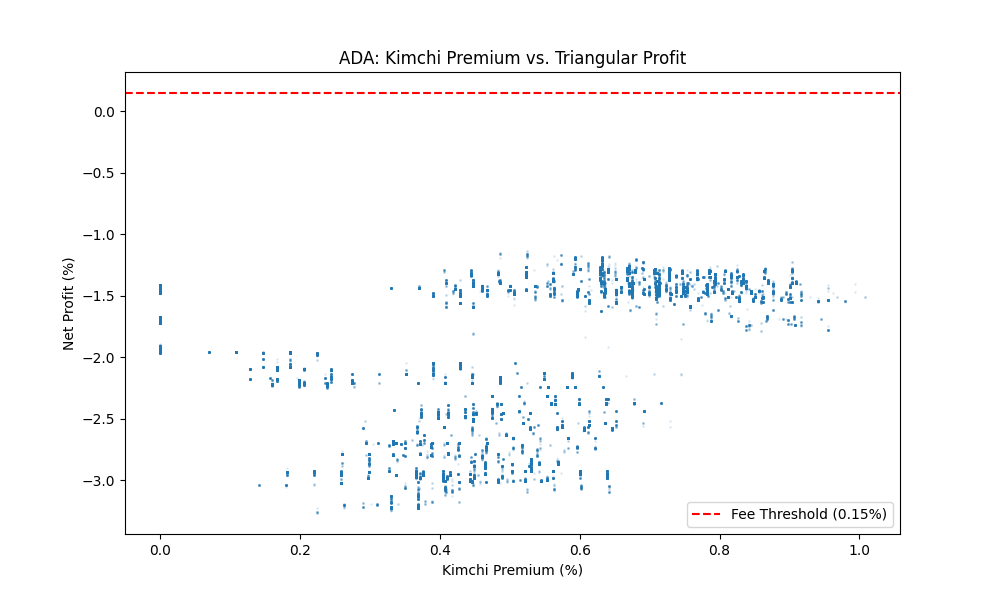
\includegraphics[width=0.95\textwidth]{ada_analysis.png}
    \caption{ADA compressed-history: kimchi premium vs triangular net profit.}
\end{figure}

\subsection{Full-Timeline Diagnostic}
\noindent Figure 2 expands the same system into full timeline resolution and overlays fee-threshold context. This higher-resolution view is useful for evaluating whether short-lived spikes approach the baseline barrier closely enough to challenge the no-edge interpretation. The figure shows that while localized upward excursions occur, they do not form sustained runs at or above the primary execution threshold.

\noindent The full-timeline perspective also makes persistence structure visually plausible: neighboring minutes tend to occupy similar route-profit regimes, consistent with the high lag-1 autocorrelation reported earlier. Crucially, this persistence appears to operate within predominantly sub-threshold states, reinforcing the distinction between \emph{state persistence} and \emph{executable-edge persistence}.

\begin{figure}[H]
    \centering
    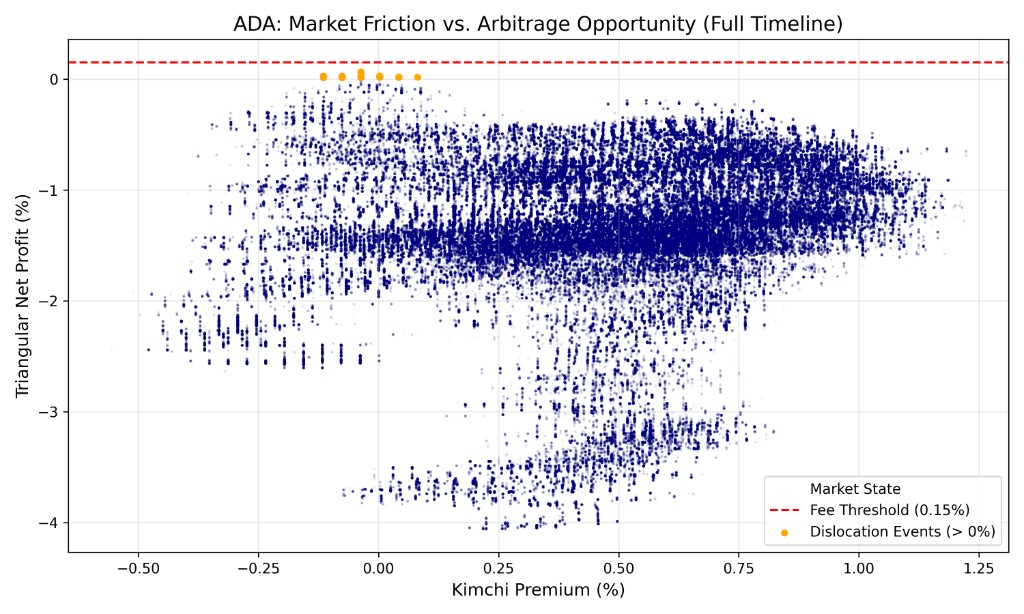
\includegraphics[width=0.95\textwidth]{ada_full_analysis.png}
    \caption{ADA full timeline: market friction vs arbitrage opportunity with fee threshold overlay.}
\end{figure}

\subsection{Takeaway}
The visualization evidence is directionally consistent with the statistical findings. Both compressed and full-resolution views show an active dislocation environment with nontrivial state movement, yet no convincing visual concentration of fee-cleared triangular opportunity. The figures therefore function as qualitative corroboration of the quantitative conclusion: in this sample, internal route states are dynamic but remain mostly trapped below practical execution barriers.

\section{Interpretation}
\subsection{Purpose}
This section synthesizes the empirical results into an economic interpretation of market behavior under the tested execution model. The central task is to explain why visible dislocation can coexist with absent fee-cleared opportunity, and to clarify what conclusions are justified versus overstated.

\subsection{Primary Interpretation}
Across all prior sections, the same structural pattern appears: the market exhibits active microstructure state movement, yet actionable triangular edge remains below practical barriers. This is consistent with a high-efficiency internal conversion system in which local route states are continuously re-equilibrated before they can generate persistent, friction-surviving opportunities.

The key point is that ``dislocation'' and ``executable arbitrage'' are not equivalent objects. Kimchi premium captures cross-venue macro divergence pressure; triangular net-profit captures internal route convertibility after local frictions. A market can therefore look dislocated in macro space while remaining locally efficient in route space. The present sample aligns with that configuration.

\subsection{Mechanism-Level Reading}
The observed evidence can be read through a friction-dominance mechanism. First, three-leg path completion compounds costs, so small gross advantages are rapidly absorbed by route-level fees. Second, short-horizon persistence indicates state continuity, but this continuity is centered in negative territory. Third, direction and asset heterogeneity produce relative ranking differences without crossing into absolute tradability. Together, these features produce a system where positive gross snapshots may occur, but the net executable tail remains effectively truncated.

\subsection{What the Results Do \emph{Not} Claim}
The results do not prove that arbitrage is impossible in all KRW-linked regimes, nor that no strategy can ever profit under different latency, depth access, or fee conditions. They also do not establish a universal law across market cycles. The claims are conditional: for this sample window, this route specification, and this friction model, persistent fee-cleared edge is not observed even in optimistic aggregation.

\subsection{Practical Implication}
For execution, the implication is conservative: baseline deployment aimed at minute-level fee-cleared triangular capture is unlikely to realize stable edge under the measured conditions. For research, the implication is constructive: state dynamics are nontrivial and potentially useful for regime monitoring, transition modeling, and risk diagnostics, even when direct arbitrage extraction is absent.

\subsection{Takeaway}
The empirical picture is best summarized as \emph{dynamic but internally efficient}. The system exhibits meaningful short-horizon structure, but not in a form that survives realistic execution friction. This interpretation motivates the remaining sections on implementation context, limitations, and future model extensions rather than immediate strategy deployment.

\section{Infrastructure Summary}
\subsection{Purpose}
This section documents the computational pipeline used to produce the empirical results, figures, and manuscript artifacts. The purpose is not merely operational convenience: reproducibility is part of the scientific claim. If the path from raw export to reported inference is not transparent, the falsification logic developed in earlier sections cannot be independently audited.

\subsection{Pipeline Architecture}
The workflow follows a linear but inspectable structure: (i) ingest/export data snapshot, (ii) compute diagnostic statistics and figures, (iii) render manuscript source, and (iv) compile to a fixed PDF artifact. This architecture is intentionally simple so that each transformation layer can be inspected and rerun without hidden state.

\begin{table}[H]
\centering
\caption{Pipeline components}
\begin{tabular}{l l}
\toprule
Component & Description \\
\midrule
Data source & \texttt{arb\_data\_export.csv} from edge-node capture \\
Core scripts & \texttt{generate\_plot.py}, \texttt{generate\_paper.py} \\
Paper source & \texttt{crypto\_kimchi\_draft\_v2.tex} \\
Compiler & \texttt{pdflatex} (double pass for TOC) \\
\bottomrule
\end{tabular}
\end{table}

\subsection{Reproducibility and Auditability}
Each component in Table 6 serves a specific audit role. The CSV export is the immutable data boundary for this draft version. The Python scripts provide deterministic transformation logic for plots and derived summary outputs. The LaTeX source is the human-readable specification of reported claims, equations, and tables. The \texttt{pdflatex} compile step generates the final research artifact with traceable build logs.

This separation improves error localization. If a numerical discrepancy is discovered, the issue can be isolated to data boundary, transformation logic, or manuscript rendering layer, rather than requiring full-pipeline re-interpretation. In practice, this is essential for short-horizon microstructure work where small alignment mistakes can materially alter tail-frequency conclusions.

\subsection{Operational Reliability Notes}
The current pipeline is designed for transparent iteration rather than production-grade orchestration. It prioritizes interpretability and editability over maximal automation. As a result, it is well-suited for rapid hypothesis testing and draft refinement, but future versions should add explicit environment pinning, checksum-based input validation, and scripted end-to-end build wrappers for stronger long-run reproducibility guarantees.

\subsection{Takeaway}
The infrastructure in this draft is sufficient for independent regeneration of all reported results from the declared export boundary, and therefore supports the paper's reproducibility standard at preprint stage. Strengthening this layer in later versions will primarily improve scale and robustness, not alter the current empirical interpretation.

\section{Limitations}
\subsection{Purpose}
The preceding sections provide internally consistent evidence for high short-horizon execution efficiency under the tested setup. This section defines the boundaries of that claim. The goal is to prevent over-interpretation by making explicit which conclusions are robust in-sample and which remain conditional on data window, friction model, and market-access assumptions.

\subsection{Sample-Horizon Constraint}
The analysis window spans roughly ten days. This horizon is sufficient to test whether strong fee-cleared edge appears in the observed regime, but it is insufficient for full-cycle inference across structurally different volatility states, liquidity regimes, and policy-event environments. As a result, persistence and regime findings should be read as local-state evidence, not long-run invariants of KRW-linked microstructure.

\subsection{Execution-Model Abstraction}
The baseline profitability framework is fee-aware but still stylized. It does not explicitly model queue position uncertainty, partial fills, depth depletion during leg sequencing, or path-dependent slippage under burst conditions. These omissions are directionally conservative for arbitrage claims: adding realistic micro-execution friction would generally reduce, not increase, executable tail mass. Nonetheless, the current model should be interpreted as a lower-bound realism layer rather than a full fill-engine simulator.

\subsection{Latency and Synchronization Risk}
Minute-level aggregation mitigates microsecond noise but does not eliminate asynchronous-leg bias. Even with server-time alignment, residual timing mismatch between route legs can create apparent transient edge that would vanish under stricter synchronized execution assumptions. Conversely, alignment smoothing can also mask ultra-short opportunities that are inaccessible without superior infrastructure. Therefore, the current timing model captures practical monitoring resolution, not exchange-colocated execution truth.

\subsection{Data Integrity and Transport Effects}
The dataset shows limited panel imbalance (e.g., XRP reverse-direction row deficit), likely driven by websocket throttling, transport jitter, or transient route reconstruction gaps. These effects may alter extreme-tail frequency estimates in either direction depending on when data loss occurs. In this draft, missingness is reported transparently and not imputed, which avoids fabricated precision but leaves open the possibility of mild tail under- or over-counting.

\subsection{External Validity}
All quantitative conclusions are conditional on the specific exchange context, route definitions, fee schedule assumptions, and asset set used here. The results should not be generalized to other venues, pairs, or infrastructure tiers without re-estimation. In particular, different fee discounts, maker-priority access, or deeper cross-venue capital mobility could materially change threshold exceedance behavior.

\subsection{Takeaway}
The limitations do not invalidate the central in-sample finding; they define its scope. Under the observed window and stated friction assumptions, fee-cleared triangular opportunity remains unobserved at baseline thresholds. Future versions should extend horizon length, strengthen fill-path realism, and formalize missingness diagnostics to test whether this conclusion survives broader structural conditions.

\section{Open Questions and v3 Roadmap}
\subsection{Purpose}
This section converts the current draft's limitations and findings into a concrete research agenda for the next version. The goal is not to list generic future work, but to define testable extensions that can either reinforce or overturn the present no-edge conclusion under broader and more realistic conditions.

\subsection{Priority 1: Horizon Extension and Regime Stability}
The first priority is expanding the dataset from a short event window to a multi-month (ideally multi-regime) panel. This enables direct testing of whether the observed zero-exceedance behavior is stable across calm, stressed, and transition states. The core question is not whether means shift, but whether the exceedance functional $\phi(\tau)=P(\Pi^\star_t>\tau)$ remains near-zero when market state changes materially.

Concretely, version 3 should report rolling-window exceedance trajectories, confidence bands, and break-point diagnostics for the threshold ladder used in Section 7. If persistent positive clusters appear only in narrow windows, that would suggest episodic, regime-conditional tradability rather than structural inefficiency.

\subsection{Priority 2: Conditional Exceedance Modeling}
A second priority is replacing descriptive threshold counts with conditional probability modeling. The natural target is:
\begin{equation}
P(\Pi^\star_t > V_0 \mid K_t,\ \text{tick\_count}_t,\ a,\ d,\ \text{state}_t),
\end{equation}
estimated using logistic or hazard-style frameworks with robust out-of-sample validation. This shifts the paper from static falsification toward predictive inference: not just \emph{whether} exceedance is rare, but \emph{when} rare exceedance risk rises.

If conditional models still assign near-zero exceedance probability across realistic covariate ranges, the high-efficiency claim gains structural support. If a narrow covariate manifold yields meaningful probability mass, the conclusion becomes conditional and strategy design can focus on state-filtered deployment.

\subsection{Priority 3: Latency-Aware Microstructure Tests}
The current minute-level alignment should be supplemented with explicit latency-window analysis around dislocation bursts. A practical design is to compute route profitability under staggered timestamp perturbations (e.g., $\pm 1\text{s}, \pm 2\text{s}, \pm 5\text{s}$ equivalent alignment windows where available) and measure sensitivity of threshold exceedance to timing offsets.

This extension directly tests whether observed near-tail events are robust microstructure states or synchronization artifacts. A large collapse under mild timing perturbation would reinforce the interpretation that apparent edge is largely non-executable in realistic asynchronous environments.

\subsection{Priority 4: Macro-Event Coupling}
Given the macro-dislocation motivation, version 3 should integrate an event calendar (policy releases, funding/liquidity shocks, FX stress episodes) and estimate pre/post event-state transitions in both kimchi premium and route profitability. The objective is to test a coupling hypothesis: macro shock intensity may increase dislocation variance without necessarily increasing fee-cleared internal opportunity.

This event-conditioned layer would elevate the paper from static microstructure description to dynamic macro-micro linkage analysis, while preserving the executable threshold discipline that distinguishes the current draft.

\subsection{Priority 5: Executable Size and Depth Depletion}
The final high-impact extension is a route-depth-aware execution model. Current statistics are effectively infinitesimal-size diagnostics; strategy relevance requires size-aware feasibility. Version 3 should estimate realized path profitability as a function of notional size using top-of-book and, if available, depth ladder snapshots, including partial-fill and depletion penalties.

This allows conversion of binary exceedance logic into capacity curves: expected net edge as a function of trade size and latency budget. Even if small-size exceedance exists, rapid decay with size would support the same practical no-edge conclusion for deployable capital.

\subsection{Milestone Plan for v3}
To keep scope tractable, the roadmap can be executed in three milestones:
\begin{enumerate}
    \item \textbf{M1 (Data \& stability):} extend horizon, compute rolling exceedance stability diagnostics.
    \item \textbf{M2 (Modeling):} fit conditional exceedance models with strict out-of-sample testing.
    \item \textbf{M3 (Execution realism):} add latency perturbation and size/depth-aware route simulation.
\end{enumerate}
Each milestone should preserve the same core falsification criterion from Section 7 so results remain comparable across versions.

\subsection{Takeaway}
The current draft supports a strong in-sample statement: actionable fee-cleared triangular edge is unobserved under the tested setup. Section 12 defines how to pressure-test that statement rigorously in version 3. If the conclusion survives longer horizon, conditional modeling, and execution-realism upgrades, the high-efficiency interpretation becomes substantially stronger; if not, the paper naturally evolves into a state-conditional arbitrage feasibility framework.

\appendix
\section{Appendix A: Reproducibility Protocol}
\subsection{Purpose and Scope}
This appendix specifies the minimum reproducibility protocol for regenerating the draft from declared inputs. The target is deterministic regeneration of the manuscript PDF and figure assets from the project directory, using the same file lineage described in Section 10. The protocol is designed for transparency and auditability rather than high-throughput orchestration.

\subsection{Input Lineage}
The reproducibility boundary for this draft is defined by the following files:
\begin{itemize}
    \item \texttt{arb\_data\_export.csv} (data boundary)
    \item \texttt{generate\_plot.py} (figure generation)
    \item \texttt{generate\_paper.py} (optional text/table assistance pipeline)
    \item \texttt{crypto\_kimchi\_draft\_v2.tex} (manuscript source)
\end{itemize}
Derived outputs include:
\begin{itemize}
    \item \texttt{ada\_analysis.png}
    \item \texttt{ada\_full\_analysis.png}
    \item \texttt{crypto\_kimchi\_draft\_v2.pdf}
\end{itemize}
Any changes to upstream inputs should be treated as a new draft state and tracked explicitly in revision notes.

\subsection{Environment Assumptions}
The workflow assumes:
\begin{itemize}
    \item Python 3 environment capable of running local plotting scripts.
    \item A working LaTeX installation with \texttt{pdflatex}.
    \item Execution from the project root:
    \texttt{finance\_quant\_analysis/crypto\_arbitrage\_kimchi/}.
\end{itemize}
For strict reproducibility, future versions should pin package versions and archive an environment manifest. In this draft, reproducibility is procedural and file-based rather than containerized.

\subsection{Deterministic Build Steps}
Recommended regeneration sequence:
\begin{verbatim}
# 1) (Optional) regenerate paper-side helper artifacts
python3 generate_paper.py

# 2) regenerate figures
python3 generate_plot.py

# 3) compile manuscript (run twice for table of contents and references)
pdflatex -interaction=nonstopmode -halt-on-error crypto_kimchi_draft_v2.tex
pdflatex -interaction=nonstopmode -halt-on-error crypto_kimchi_draft_v2.tex
\end{verbatim}
The double compile is required to ensure stable table-of-contents rendering and consistent pagination.

\subsection{Verification Checklist}
After build completion, the following checks should pass:
\begin{enumerate}
    \item \texttt{crypto\_kimchi\_draft\_v2.pdf} is generated without LaTeX fatal errors.
    \item Both figure files are present and referenced successfully in the compiled PDF.
    \item Key threshold statements in Section 7 match source statistics:
    $\phi(0.35\%)=0$ and stricter-threshold exceedance remains zero.
    \item Table values and narrative claims remain internally consistent after regeneration.
\end{enumerate}

\subsection{Known Reproducibility Risks}
Two practical risks remain in the current workflow. First, data-export regeneration may depend on external infrastructure state (feed timing, transport stability), so regenerated datasets across different dates are not expected to be numerically identical. Second, script-level environment drift can alter plotting defaults or floating-point formatting. These risks do not invalidate the current draft but should be documented whenever results are refreshed.

\subsection{Appendix A Conclusion}
Under the stated input boundary and build procedure, the manuscript can be regenerated reproducibly at the document level. Future hardening should focus on environment pinning, checksum logging, and automated end-to-end validation scripts to elevate this protocol from preprint-grade reproducibility to production-grade research operations.

\end{document}

